\documentclass[aspectratio=169]{beamer}
%\documentclass[xcolor=pst,dvips,epic,eepic]{beamer}

\usepackage[utf8]{inputenc}
\usetheme{Singapore}
\usepackage{xcolor}
\setbeamertemplate{footline}[frame number]

%\usepackage{pgf,pgfarrows,pgfnodes,pgfautomata,pgfheaps,pgfshade}
%\usepackage[pst]{xcolor}
%\usepackage{xxcolor}
%\usepackage{../sty/mathlist}

\input{../sty/macros}

%\usepackage[french]{babel}
\usepackage{amsmath,amssymb}
%\usepackage{colortbl}
%\usepackage[english]{babel}

\usepackage{tikz}
\usetikzlibrary{positioning}

\usepackage{times}

\usepackage{ulem}

\usepackage{listings}
%\topmargin=-0.6in
\lstloadlanguages{C++}
\lstset{language=C++}
%%}

\setbeamercovered{dynamic}

\def\bxi{\boldsymbol\xi}
\def\bx{\boldsymbol{x}}
\def\bu{\boldsymbol{u}}
\def\bz{\boldsymbol{z}}
\def\bomega{\boldsymbol\omega}

%% ---------------------------------------------------------------------------
%% Scenario-tree pictures, in TikZ (no PSTricks, no auto-pst-pdf).
%% ---------------------------------------------------------------------------

% SDDP tree. #1 = level drawn in red (0 = none, 1, 2 or 3); #2-#8 = node
% labels ($x_1$; second stage; third stage), each empty for no label.
% Places a label under a tree node, unless it is empty.
\newcommand{\sddplbl}[2]{\ifx&#2&\else\node[lbl,below=1pt of #1]{#2};\fi}

\newcommand{\sddptree}[8]{%
  \ifnum#1=1 \def\cA{red}\else\def\cA{black}\fi
  \ifnum#1=2 \def\cB{red}\else\def\cB{black}\fi
  \ifnum#1=3 \def\cC{red}\else\def\cC{black}\fi
  \begin{tikzpicture}[scale=0.93,
      nd/.style={circle,draw,line width=1pt,minimum size=5.5mm,inner sep=0pt},
      lf/.style={circle,fill,inner sep=1.3pt},
      lbl/.style={font=\footnotesize,inner sep=2pt,fill=white},
      link/.style={densely dotted,line width=0.7pt}]
    % nodes
    \node[nd,draw=\cA] (s0)  at (0,0)     {};
    \node[nd,draw=\cA] (s1a) at (3,1.6)   {};
    \node[nd,draw=\cA] (s1b) at (3,-1.6)  {};
    \node[nd,draw=\cB] (s2a) at (6,2.4)   {};
    \node[nd,draw=\cB] (s2b) at (6,0.8)   {};
    \node[nd,draw=\cB] (s2c) at (6,-0.8)  {};
    \node[nd,draw=\cB] (s2d) at (6,-2.4)  {};
    \node[lf,fill=\cC] (l1) at (8.4,2.82) {};
    \node[lf,fill=\cC] (l2) at (8.4,1.98) {};
    \node[lf,fill=\cC] (l3) at (8.4,1.22) {};
    \node[lf,fill=\cC] (l4) at (8.4,0.38) {};
    \node[lf,fill=\cC] (l5) at (8.4,-0.38){};
    \node[lf,fill=\cC] (l6) at (8.4,-1.22){};
    \node[lf,fill=\cC] (l7) at (8.4,-1.98){};
    \node[lf,fill=\cC] (l8) at (8.4,-2.82){};
    % edges
    \draw[\cA] (s0)  -- (s1a);  \draw[\cA] (s0)  -- (s1b);
    \draw[\cB] (s1a) -- (s2a);  \draw[\cB] (s1a) -- (s2b);
    \draw[\cB] (s1b) -- (s2c);  \draw[\cB] (s1b) -- (s2d);
    \draw[\cC,dashed] (s2a) -- (l1);  \draw[\cC,dashed] (s2a) -- (l2);
    \draw[\cC,dashed] (s2b) -- (l3);  \draw[\cC,dashed] (s2b) -- (l4);
    \draw[\cC,dashed] (s2c) -- (l5);  \draw[\cC,dashed] (s2c) -- (l6);
    \draw[\cC,dashed] (s2d) -- (l7);  \draw[\cC,dashed] (s2d) -- (l8);
    % nonanticipativity links between siblings
    \draw[link] (s1a) -- (s1b);
    \draw[link] (s2a) -- (s2b);  \draw[link] (s2c) -- (s2d);
    \draw[link] (l1) -- (l2);    \draw[link] (l3) -- (l4);
    \draw[link] (l5) -- (l6);    \draw[link] (l7) -- (l8);
    % node labels (skipped when empty)
    \sddplbl{s0}{#2}
    \sddplbl{s1a}{#3}\sddplbl{s1b}{#4}
    \sddplbl{s2a}{#5}\sddplbl{s2b}{#6}
    \sddplbl{s2c}{#7}\sddplbl{s2d}{#8}
    % stage identifiers
    \node[font=\footnotesize] at (0,-3.9)   {First stage};
    \node[font=\footnotesize] at (3,-3.9)   {Second stage};
    \node[font=\footnotesize] at (6,-3.9)   {Third stage};
    \node[font=\footnotesize] at (8.4,-3.9) {\ldots};
  \end{tikzpicture}}

% Full scenario tree: one root, four second-stage nodes, sixteen leaves.
\newcommand{\fullscenariotree}{%
  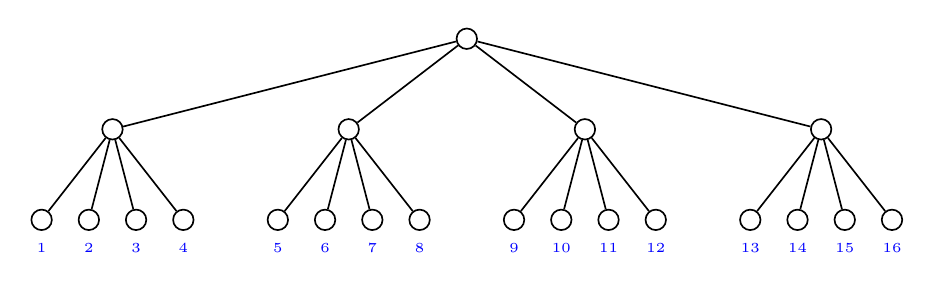
\begin{tikzpicture}[scale=1,
      nd/.style={circle,draw,line width=0.6pt,minimum size=2.6mm,inner sep=0pt}]
    \node[nd] (r) at (0,0) {};
    \foreach \i/\gx in {1/-4.5,2/-1.5,3/1.5,4/4.5} {
      \node[nd] (g\i) at (\gx,-1.15) {};
      \draw[line width=0.6pt] (r) -- (g\i);
      \foreach \j/\dx in {1/-0.9,2/-0.3,3/0.3,4/0.9} {
        \pgfmathtruncatemacro{\num}{4*(\i-1)+\j}
        \node[nd] (t\num) at (\gx+\dx,-2.3) {};
        \draw[line width=0.6pt] (g\i) -- (t\num);
        \node[font=\tiny\bfseries,text=blue,below=1pt of t\num] {$\num$};
      }
    }
  \end{tikzpicture}}

% Nonanticipativity: the same tree bundled into three stage-two groups.
\newcommand{\bundletree}{%
  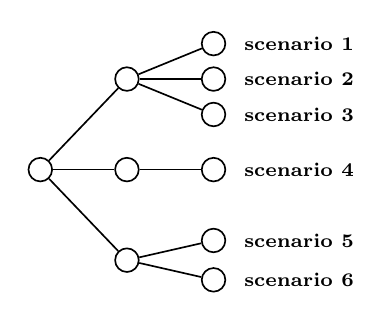
\begin{tikzpicture}[scale=1,
      nd/.style={circle,draw,line width=0.6pt,minimum size=3mm,inner sep=0pt},
      lbl/.style={font=\scriptsize\bfseries,right=3pt}]
    \node[nd] (r) at (0,0) {};
    \foreach \i/\gy in {1/1.15,2/0,3/-1.15} { \node[nd] (g\i) at (1.1,\gy) {}; \draw[line width=0.6pt] (r) -- (g\i); }
    \foreach \k/\gi/\ly in {1/1/1.6,2/1/1.15,3/1/0.7,4/2/0,5/3/-0.9,6/3/-1.4} {
      \node[nd] (s\k) at (2.2,\ly) {};
      \draw[line width=0.6pt] (g\gi) -- (s\k);
      \node[lbl] at (s\k.east) {scenario \k};
    }
  \end{tikzpicture}}

% Nonanticipativity, nodal view: six scenarios x three periods, with the
% doubled bars marking the variables that must be bundled together.
\newcommand{\nodalbundles}{%
  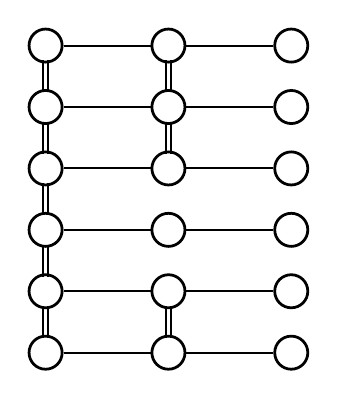
\begin{tikzpicture}[scale=0.78,
      nd/.style={circle,draw,line width=1pt,minimum size=4.2mm,inner sep=0pt}]
    \foreach \r in {0,1,2,3,4,5} {
      \foreach \c/\x in {a/0,b/2,c/4} { \node[nd] (n\r\c) at (\x,\r) {}; }
      \draw[line width=0.7pt] (n\r a) -- (n\r b);
      \draw[line width=0.7pt] (n\r b) -- (n\r c);
    }
    % left column: every consecutive pair is bundled
    \foreach \r/\rr in {5/4,4/3,3/2,2/1,1/0} {
      \draw[line width=0.7pt] (-0.04,\r-0.24) -- (-0.04,\rr+0.24);
      \draw[line width=0.7pt] ( 0.04,\r-0.24) -- ( 0.04,\rr+0.24);
    }
    % middle column: only within a stage-two group
    \foreach \r/\rr in {5/4,4/3,1/0} {
      \draw[line width=0.7pt] (1.96,\r-0.24) -- (1.96,\rr+0.24);
      \draw[line width=0.7pt] (2.04,\r-0.24) -- (2.04,\rr+0.24);
    }
  \end{tikzpicture}}

\title[Multi-stage problems]{Stochastic programming\\Multi-stage problems}

\author[Fabian Bastin]{Fabian Bastin \\ \url{bastin@iro.umontreal.ca} \\ Université de Montréal -- CIRRELT -- IVADO -- Fin-ML}

\date{}

\setbeamertemplate{footline}[frame number]

\begin{document}

\frame{\titlepage}

\begin{frame}
\frametitle{Motivation: example}

\begin{itemize}
\item
Assume that we invest in the market.
We would like to reach a nominal goal $G$ after $Y$ years.
\item
The portfolio is rebalanced every $v$ years, so there are $T = Y/v$ times where we have to decide what are the investments to do.\\
There are $T$ stages in our problem.
\item
We face a space of $N$ investment decisions (i.e. we have $N$ possible actions); we have a set $\mathcal{T} = \lbrace 1, 2,\ldots, T \rbrace$ of investment periods.
\item
If we go over the target $G$, we will have an interest rate $q$ on the surplus.
\item
If we do not meet the target, we have to borrow the difference at an interest $r$.
\item
The initial wealth is $b$.
\end{itemize}

\end{frame}

\begin{frame}
\frametitle{Variables}

\begin{itemize}
\item
$x_{it}$, $i \in N$, $t \in \mathcal{T}$: amount of money to invest in action $i$ during the period $t$;
\item
$y$: excess amount at the end of the horizon;
\item
$w$: lack of money at the end of the horizon;
\item
In the current framework, we aim to take the corrective actions in order to reach the target of $G$ dollars.
\end{itemize}

\end{frame}

\begin{frame}
\frametitle{Deterministic formulation}

\begin{align*}
\max\ qy & - rw\\
\mbox{s.t. } \sum_{i \in N} x_{i1} & = b,\\
\sum_{i \in N} \omega_{it}x_{i,t-1} & = \sum_{i \in N} x_{it}, \quad
\forall t \in \mathcal{T} \backslash 1, \\
\sum_{i \in N} \omega_{iT}x_{iT} - y + w & = G,\\
x_{it} & \geq 0, \quad \forall i \in N,\ t \in \mathcal{T}, \\
y, w & \geq 0.
\end{align*}

\end{frame}

\begin{frame}
\frametitle{Random returns}

\begin{itemize}
\item
The investment returns can be viewed as random variables, as we do not know their realizations in advance.
\item
Imagine that for each action, at each time $t$, there are $R$ possible realizations.
\item
The scenarios are made of all the possible sequences of realizations.
\end{itemize}

Example: assume $R = 4$ and $T = 3$. Scenarios:
\begin{small}
\begin{center}
\begin{tabular}{ccc}
\hline
$t = 1$ & $t = 2$ & $t = 3$ \\
\hline
1 & 1 & 1 \\
1 & 1 & 2 \\
1 & 1 & 3 \\
1 & 1 & 4 \\
1 & 2 & 1 \\
\vdots & \vdots & \vdots \\
4 & 4 & 4 \\
\end{tabular}
\end{center}
\end{small}

\end{frame}

\begin{frame}
\frametitle{Stochastic program formulation}

\begin{itemize}
\item
Let $x_{its}$, $t \in \mathcal{T}$, $s \in S$ be the amount to invest in action $i$ during the period $t$ in scenario $s$;
\item
$y_s$: excess amount at the end of the horizon for scenario $s$;
\item
$w_s$: lack of money at the end of the horizon for scenario $s$.
\item
Let $\omega_{it}$ be the random return; it can be seen as function of the scenario $s$.
\end{itemize}

\end{frame}

\begin{frame}
\frametitle{Stochastic version}

\begin{align*}
\max\ \sum_{s=1}^S p_s(qy_{\red s} & - rw_{\red s})\\
\mbox{s.t. } \sum_{i \in N} x_{i1} & = b,\\
\sum_{i \in N} \omega_{it{\red s}}x_{i,t-1,{\red s}} & = \sum_{i \in
  N} x_{it{\red s}}, \quad \forall t \in \mathcal{T} \backslash 1,
{\red \forall s \in S} \\
\sum_{i \in N} \omega_{iT{\red s}}x_{iT} - y_{\red s} + w_{\red s} & = G,
\quad {\red \forall s \in S}, \\
x_{it{\red s}} & \geq 0, \quad \forall i \in N,\ t \in \mathcal{T},
{\red \forall s \in S},\\
y_{\red s}, w_{\red s} & \geq 0 \quad {\red \forall s \in S}.
\end{align*}

\end{frame}

\begin{frame}
\frametitle{Scenario tree}

Conceptually, the sequence of events can be arranged in a tree.
There is one leaf per scenario.
\begin{center}
\fullscenariotree
\end{center}

The scenarios can have different probabilities, the variables can be correlated,\ldots

\end{frame}

\begin{frame}
\frametitle{Non-anticipativity}

\begin{itemize}
\item
The conversion between the deterministic model and the stochastic version is easy\ldots
\item
but the built model is wrong!!!
\item
We have to enforce the {\red non-anticipativity}:
\end{itemize}

Let $S_s^t$ be the set of scenarios that are identical to scenario $s$ at time $t$.
We have to guarantee that
\[
x_{its} = x_{its'},\ \forall i \in N,\ \forall t \in T,\ \forall s \in
S,\ \forall s' \in S_s^t.
\]

\end{frame}

\begin{frame}
\frametitle{Non-anticipativity (cont'd)}

Equivalently,
\[
\left( \sum_{s' \in S_s^t} p'_s \right) x_{its} = \sum_{s' \in S_s^t} p'_s x_{its'} \quad \forall\ i,t,s,
\]
or
\begin{align*}
 x_{its}
&= \frac{\sum_{s' \in S_s^t} p'_s x_{its'}}{\sum_{s' \in S_s^t} p'_s} \quad \forall\ i,t,s \\
&= E[ x_{its'} | s' \in S_s^t ] \quad \forall\ i,t,s.
\end{align*}

The amount invested in scenario $s$, multiplied by the probability to reach a scenario equivalent to $s$, has to be equal to the expected amount that would be invested in any scenario equivalent to $s$.

There are many formulations of these conditions!

\end{frame}

\begin{frame}
	\frametitle{Back to the scenario tree}
	
	\begin{itemize}
		\item
		We have to enforce nonanticipativity as we have created copies of the variables for each scenario, at each period.
		Graphically:
	\end{itemize}
	\begin{minipage}{0.45\textwidth}
		\begin{center}
			\bundletree
		\end{center}
	\end{minipage}
	\hfill
	\begin{minipage}{0.45\textwidth}
		\begin{center}
			\nodalbundles
		\end{center}
	\end{minipage}
   	
\end{frame}

\begin{frame}
\frametitle{Nodal approach}

\begin{itemize}
\item
We can also create a vector of variables for each node in the tree.
\item
This vector corresponds to what should be our decision given the known realizations of the random variables upon this stage (i.e. at this node).
\item
Index the nodes by $l = 1,2,\ldots,\mathcal{L}$.
\item
We have to know the ancestor of each node.
Let $A(l)$ be the ancestor of node $l \in \mathcal{L}$ in the scenarios tree.
\end{itemize}

\end{frame}

\begin{frame}
\frametitle{Reformulation}

\begin{alignat*}{2}
\max\ & \sum_{s \in S} p_s (qy_{s} & - rw_{s})\\
\mbox{s.t. } & \sum_{i \in N} x_{i1} & = b,\\
& \sum_{i \in N} \omega_{il}x_{i,A(l)} & = \sum_{i \in N} x_{il}, \quad \forall l \in \mathcal{L} \backslash 1, \\
& \sum_{i \in N} w_{iA(s)}x_{iA(s)} - y_{s} + w_{s} & = G,
\quad {\forall s \in S}, \\
& x_{il} & \geq 0, \quad \forall i \in N,\ \forall l \in \mathcal{L},\\
& y_{s}, w_{s} & \geq 0 \quad {\forall s \in S}.
\end{alignat*}

\end{frame}

\begin{frame}
\frametitle{Multi-period production planning}

\begin{itemize}
\item
A firm produces various different goods.
\item
Resources (for instances manual and machine work hours) are required.
We assume that these requirements are known for each product.
\item
The demand must be met at the end of each period, but this demand is not perfectly known.
\item
A too large or too small inventory induces costs (storage, additional purchases to satisfy the demand,\ldots).
\item
It is possible to add machine and work hours, within predefined limits.
\item
There is a hiring and firing cost related to changes in the workforce.
\end{itemize}

\end{frame}

\begin{frame}
\frametitle{Decision problem}

\begin{itemize}
\item
We have to decide now on
\begin{itemize}
\item
the quantity of each product to manufacture during each period;
\item
the additional capacity to use during each period;
\item
to hire or to fire staff during each period;
\end{itemize}
\item
A random demand occurs. Conceptually, this happens at each period.
\item
After having observed the random demands, we can decide on how to stock the products in the inventory, or to buy from an external source.
\end{itemize}

\end{frame}

\begin{frame}
\frametitle{Definitions}

\begin{enumerate}
\item
{\red Sets}:
\begin{itemize}
\item
$T$: number of periods, also seen as a set;
\item
$N$: products;
\item
$M$: resources.
\end{itemize}
\item
{\red Variables}:
\begin{itemize}
\item
$x_{jt}$: production of product $j \in N$ during the period $t \in T$;
\item
$u_{it}$: additional amount of resource $i \in M$ to buy during the period  $t \in T$;
\item
$z_{t-1,t}^+$, $z_{t-1,t}^-$: planned augmentation or reduction of the labor force;
\item
$y_{j,t}^+$, $y_{j,t}^-$: surplus, deficit of product $j \in N$ at the end of the period $t \in T$.
\end{itemize}
\end{enumerate}

\end{frame}

\begin{frame}
\frametitle{Parameters}

\begin{itemize}
\item
All the above variables have associated costs $(\alpha,\,\beta,\,\gamma,\,\delta)$.
\item
$\omega_{jt}$: demand of product $j \in N$ during the period $t
\in T$.
\item
$U_{it}$: upper bound on $u_{it}$.
\item
$a_{ij}$: amount of resource $i \in M$ required to produce one unit of the good $j \in N$.
\item
$b_{it}$: amount of resource $i \in M$ available at time $t \in T$.
\end{itemize}

\end{frame}

\begin{frame}
\frametitle{Model}

{\small
\begin{multline*}
\min \sum_{j \in N} \sum_{t \in T} \alpha_{jt} x_{jt} + \sum_{i \in M}
\sum_{t \in T} \beta_{it} u_{it} + \sum_{t \in T\backslash 1} \left(
  \gamma^+_{t-1,t} z^+_{t-1,t} + \gamma^-_{t-1,t} z^-_{t-1,t} \right) \\
+ E_{\bomega} \left[ \min \left( \sum_{j \in N} \sum_{t \in T}
    ( \delta_{jt}^+y_{jt}^+ + \delta_{jt}^-y_{jt}^- ) \right) \right],
\end{multline*}
such that
\begin{align*}
\sum_{j \in N} a_{ij} x_{jt} & \leq b_{it}+u_{it} \quad \forall i \in
M,\ \forall t \in T,\\
u_{it} & \leq U_{it} \qquad \forall i \in M,\ \forall t \in T,\\
z^+_{t-1,t} - z^-_{t-1,t} &= \sum_{j \in N} a_{jt}(x_{jt} - x_{j,
  t-1}) \quad \forall t \in T\backslash 1, \\
x_{jt} + y_{j,t-1}^+ - y_{jt}^+ + y_{jt}^- &= \omega_{jt} \qquad
\forall j \in N,\ \forall t \in T\ \mbox{(demand satisfaction)},\\
\end{align*}
}
\end{frame}

\begin{frame}
\frametitle{Extended form of the recourse model}

{\small
\begin{multline*}
\min \sum_{j \in N} \sum_{t \in T} \alpha_{jt} \bx_{jt} + \sum_{i \in M}
\sum_{t \in T} \beta_{it} \bu_{it} + \sum_{t \in T\backslash 1} \left(
  \gamma^+_{t-1,t} \bz^+_{t-1,t} + \gamma^-_{t-1,t} \bz^-_{t-1,t} \right) \\
+ {\red \sum_{s \in S}}\sum_{j \in N} \sum_{t \in T} p_s
    ( \delta_{jt}^+y_{jt{\red s}}^+ + \delta_{jt}^-y_{jt{\red s}}^- ),
\end{multline*}
such that
\begin{align*}
\sum_{j \in N} a_{ij} \bx_{jt} & \leq b_{it}+\bu_{it} \quad \forall i \in
M,\ \forall t \in T,\\
\bu_{it} & \leq U_{it} \qquad \forall i \in M,\ \forall t \in T,\\
\bz^+_{t-1,t} - \bz^-_{t-1,t} &= \sum_{j \in N} a_{jt}(\bx_{jt} - \bx_{j,
  t-1}) \quad \forall t \in T\backslash 1, \\
\bx_{jt} + y_{j,t-1,{\red s}}^+ - y_{jt{\red s}}^+ + y_{jt{\red s}}^- &= \omega_{jt{\red s}} \qquad
\forall j \in N,\ \forall t \in T,\\
\mbox{nonanticipativity }& \mbox{constraints}.
\end{align*}
}
\end{frame}

\begin{frame}
\frametitle{Potential solution techniques}

Adapted from Jalal Kazempour, \url{https://www.jalalkazempour.com/teaching}

\begin{itemize}
\item 
\textcolor{red}{Direct solution}:
computational issues
\item 
\textcolor{red}{Linear decision rules}: 
a non‐decomposition approach with approximation.
Assumption of linear dependency between decision variables and uncertain
parameters. Using this approximation, the number of constraints and variables grows
only linearly with the number of stages.
\item 
\textcolor{red}{Nested Benders decomposition}: a decomposition approach based on fixing complicating variables.
\item 
\textcolor{red}{Lagrangian relaxation}: a decomposition approach based on relaxing the complicating (non‐anticipativity) constraints.
\end{itemize}

\end{frame}

\begin{frame}
\frametitle{Nested Benders decomposition}

\begin{itemize}
	\item 
Nested Benders decomposition, also called the \emph{multistage L-shaped method}, generalizes the classical two-stage Benders decomposition to stochastic linear programs with multiple decision stages.
\item 
It recursively applies (two-stage) Benders decomposition on a scenario tree, where each stage generates cuts for its parent stage.
\end{itemize}

\end{frame}

\begin{frame}
\frametitle{Model structure}

Consider a $T$-stage stochastic linear program of the form:
\begin{align*}
	\min_{x_1, \ldots, x_T} \quad & \mathbb{E} \left[ \sum_{t=1}^T c_t(\xi_t)^\top x_t \right] \\
	\text{s.t.} \quad & A_1 x_1 = b_1, \quad x_1 \ge 0, \\
	& A_t x_t = b_t(\xi_t) - T_t(\xi_t) x_{t-1}, \quad x_t \ge 0, \quad t = 2, \ldots, T.
\end{align*}
Each $\xi_t$ represents the random information revealed at stage $t$, defining a scenario tree.

\end{frame}

\begin{frame}
\frametitle{Recursive value functions}

Define recursively the cost-to-go function:
\begin{align*}
	Q_t(x_{t-1}, \xi_t) & = 
	\min_{x_t \ge 0} c_t(\xi_t)^\top x_t + \EE[ Q_{t+1}(x_t, \xi_{t+1}) \mid \xi_t ] \\
	& \mbox{s.t. } A_t x_t = b_t(\xi_t) - T_t(\xi_t) x_{t-1},
\end{align*}
with $Q_{T+1} \equiv 0$. The goal is to approximate $Q_t$ at each stage with a piecewise-linear function constructed from Benders cuts.

\mbox{}

Assume for simplicity the recourse is complete.

\end{frame}

\begin{frame}
\frametitle{Cut generation (optimality cut)}

At iteration $k$, for each scenario $\xi_t^s$, the subproblem is solved:
\begin{align*}
	\min_{x_t^s \ge 0} \quad & c_t^s{}^\top x_t^s + \sum_{s'} p_{s'|s} \theta_{t+1}^{s'} \\
	\text{s.t.} \quad & A_t^s x_t^s = b_t^s - T_t^s x_{t-1}^{p(s)}.
\end{align*}

Let $\pi_t^s$ denote the optimal duals for the equality constraints. Then the expected cost-to-go can be approximated as:
\begin{align}
	Q_t(x_{t-1}) \ge \alpha_t + \beta_t^\top x_{t-1},
\end{align}
where
\begin{align}
	\alpha_t = \sum_s p_s (\pi_t^s)^\top b_t^s, \qquad
	\beta_t = - \sum_s p_s (\pi_t^s)^\top T_t^s.
\end{align}
These $(\alpha_t, \beta_t)$ pairs define the Benders cuts for the parent stage.

\end{frame}

\begin{frame}
	\frametitle{Algorithm outline}

\begin{enumerate}
	\item \textbf{Initialization:} Start with initial lower approximations $\theta_t$ for all stages.
	\item \textbf{Forward pass:} Fix first-stage decision $x_1$ and recursively compute trial points $x_t$ through the scenario tree.
	\item \textbf{Backward pass:} Starting from the leaves, solve subproblems, extract duals, and form cuts for each parent node.
	\item \textbf{Master problem update:} Add the new cuts to each parent’s master problem and reoptimize.
	\item \textbf{Convergence:} Stop when the expected gap between upper and lower bounds is within tolerance.
\end{enumerate}

\end{frame}

\begin{frame}
\frametitle{Remarks}

\begin{itemize}
	\item The algorithm is naturally parallelizable across scenarios.
	\item Feasibility cuts are added if subproblems are infeasible, similar to two-stage Benders.
	\item For convex piecewise-linear approximations, monotonic convergence to the optimal policy is guaranteed.
\end{itemize}

\end{frame}

\begin{frame}
	\frametitle{Illustration}
	
	\begin{center}
		\sddptree{0}{$x_1$}{}{}{}{}{}{}
	\end{center}
	
\end{frame}

\begin{frame}
	\frametitle{Step 1: forward pass}
	
	\begin{center}
		\sddptree{1}{$x_1$}{}{}{}{}{}{}
	\end{center}
	
\end{frame}

\begin{frame}
\frametitle{Step 1: forward pass}

Solve
\begin{align*}
\min_{x_1, \theta_1}\ & c_1^Tx_1 + \theta_1 \\
\mbox{s.t. } & A_1x_1 = b_1 \\
& \theta_1 \geq \theta_{1,\min} \\
& \text{feasibility and optimality cuts} \\
& x_1 \geq 0.
\end{align*}

\end{frame}

\begin{frame}
	\frametitle{Step 2: forward pass}
	
	\begin{center}
		\sddptree{2}{$x_1$}{$x_{2,1}$}{$x_{2,s_{n_2}}$}{}{}{}{}
	\end{center}
	
\end{frame}

\begin{frame}
	\frametitle{Step 2: forward pass}
	
	Solve
	\begin{align*}
		\min_{x_{2,i}, \theta_{2,i}}\ & c_{2,i}^Tx_{2,i} + \theta_{2,i} \\
		\mbox{s.t. } % & A_{1,i}x_{1,i} = b_{1,i} \\
		& A_{2,i}x_{2,i} = h_{2,i}-T_{2,i}x_{0} \\
		& \theta_{2,i} \geq \theta_{2,i,\min} \\
		& \text{feasibility and optimality cuts} \\
		& x_{2,i} \geq 0.
	\end{align*}
\end{frame}


\begin{frame}
	\frametitle{Step 3: forward pass}
	
	\begin{center}
		\sddptree{3}{$x_1$}{$x_{2,1}$}{$x_{2,s_1}$}{$x_{3,1}$}{$x_{3,s_i}$}{$x_{3,s_m}$}{$x_{3,s_{n_3}}$}
	\end{center}
	
\end{frame}

\begin{frame}
\frametitle{Step 2: backward pass}

The newly formed cuts are added to the Step 2 program and we solve again the program to determine cuts on the second-stage program.
	
\end{frame}

\begin{frame}
	\frametitle{Step 2: backward pass}
	
	\begin{center}
		\sddptree{2}{$x_1$}{$x_{2,1}$}{$x_{2,s_{n_2}}$}{}{}{}{}
	\end{center}
	
\end{frame}

\begin{frame}
\frametitle{Step 1: backward pass}

The newly formed cuts are added to the Step 1 program.

\mbox{}

This forms a new master program for the first stage, that is solved again in the forward pass.

\end{frame}
	
\begin{frame}
	\frametitle{Step 1: backward pass}
	
	\begin{center}
		\sddptree{1}{$x_1$}{}{}{}{}{}{}
	\end{center}

\end{frame}

\begin{frame}
\frametitle{Scenario tree}

The main issue is the construction of the scenario tree that is growing exponentially at each stage, and so the number of subproblems.

\mbox{}

The stochastic dual dynamic programming algorithm aims to solve the problem on a lattice rather than a tree, under the assumption that the underlying random process is Markovian.

\mbox{}

The augmented Lagrangian approaches will still rely on the scenario tree, but will consider the relaxation on the nonanticipativity constraints rather than solve a succession a two-stage problems. This limits the number of subproblems to the number of scenarios and can handle non-Markovian processes. The drawback is that it can take many iterations to restore non-anticipativity.

\end{frame}

\end{document}
